\chapter{Implementacija i korisničko sučelje}
		
		
		\section{Korištene tehnologije i alati}
		
			Komunikacija u timu ostvarena je pomoću platforme Discord\footnote{\url{https://discord.com}} koja nudi opcije tekstualnog dopisivanja, glasovnog poziva i videopoziva. U serveru našeg projektnog tima postojalo je nekoliko kanala koji su se bavili različitim temama (back-end, front-end, dokumentacija…) što nam je pomoglo u podjeli posla i filtriranju zadataka. Za izradu UML dijagrama koristili smo se aplikacijom Astah\footnote{\url{https://astah.net}} pomoću koje smo vrlo jednostavno napravili željene dijagrame i time pokazali ideju projektnog zadatka, kao i način rada naše aplikacije. Za rad s LaTeX-om poslužio nam je Texmaker\footnote{\url{https://www.xm1math.net/texmaker}}. Kao sustav za upravljanje izvornim kodom koristili smo Git\footnote{\url{https://git-scm.com}}. Udaljeni repozitorij projekta dostupan je na web platformi GitHub\footnote{\url{https://github.com}}. \\
Za razvojno okruženje koristili smo Visual Studio Code\footnote{\url{https://code.visualstudio.com}} i IntelliJ IDEA\footnote{\url{https://jetbrains.com/idea}}. VSC nudi široku podršku za jezike i ekstenzije, integraciju s Git-om i različitim alatima i servisima (Docker\footnote{\url{https://docker.com}}) te snimanje koraka za debuggiranje. Također, dolazi s ugrađenom podrškom za JavaScript i TypeScript. IntelliJ IDEA nudi naprednu podršku za pisanje koda (Code Assistance), odličan debugger, refaktoriranje koda te podršku za različite tehnologije (Spring Framework, JavaScript, HTML, CSS, TypeScript, React, SQL) i jezike (Java, Kotlin, Groovy). \\
Klijentska strana aplikacije (\textit{front-end}) napisana je React\footnote{\url{https://react.dev}}-om preko TypeScript\footnote{\url{https://typescriptlang.org}}-a i Vite.js\footnote{\url{https://vitejs.dev}}-om. Material UI\footnote{\url{https://mui.com/material-ui}} je biblioteka React komponenata koja pruža implementaciju Google-ovog Material Design koncepta u React aplikacijama, a fokusiran je na stvaranje dosljednih i intuitivnih korisničkih sučelja.\\
Poslužiteljska strana aplikacije (\textit{back-end}) napisana je u Kotlinu\footnote{\url{https://kotlinlang.org}} koristeći Spring Framework\footnote{\url{https://spring.io/projects/spring-framework}}. Kotlin omogućuje interoperabilnost s jezikom Java\footnote{\url{https://java.com/en}} (može se koristiti zajedno s njim u sklopu istog projekta te koristiti njegove biblioteke). Spring Framework je open-source radni okvir za razvoj aplikacija baziranih na Javi. On implementira inverziju kontrole (IoC), uvođenje ovisnosti (DI), Model-View-Controller (MVC), pristup podacima, sigurnost i Spring Boot. \\
Pokretanje, izvršavanje i puštanje u pogon izvršavaju se preko 3 kontejnera platforme Docker koji pokrivaju najvažnije dijelove aplikacije: back-end, front-end i PostgreSQL bazu podataka. Pri deployment-u projekta koristimo radni okvir Express.js\footnote{\url{https://expressjs.com}} za izgradnju API-ja s Node.js\footnote{\url{https://nodejs.org/en}} radnim okruženjem.

			
			\eject 
		
	
		\section{Ispitivanje programskog rješenja}
	
			
			\subsection{Ispitivanje komponenti}
			
			Komponente programskog sustava ostvaruju određenu funkcionalnost te međusobno imaju usku komunikaciju preko raznih ponuđenih sučelja. Pomoću unit testova provjeravamo ispravnost i pravilno ponašanje pojedinačnih "jedinica" komponenti, najčešće funkcija ili metoda. To su najmanji dijelovi softverskog sustava koji se mogu testirati odvojeno, a provođenjem unit testiranja poboljšavamo kvalitetu koda tijekom vremena te identificiramo eventualne probleme. \\
			
Ispitivanje komponenti ostvareno je preko JUnit radnog okvira, a proveli smo 2 vrste testova: testiranje ponašanja sustava prilikom unosa ispravnih podataka te testiranje rubnih slučajeva odnosno ponašanja sustava kod unosa neispravnih podataka.  Prilikom testiranja UserService metoda, korišteno je sučelje UserRepository uz klase User i DTO objekata koji su korišteni za entitet User. Prilikom testiranja AdService metode za dodavanje oglasa korištena su sučelja: ActivityRepository, CityRepository, AdRepository, ColorRepository, CountyRepository, ImageRepository, LocationRepository, PetRepository, SpeciesRepository, UserRepository te klase DTO objekata potrebne za kreiranje novog oglasa.\\
Proveli smo sveukupno 6 unit testova te u nastavku slijede njihovi opisi i slike kodova.

\pagebreak

\textbf{Ispitni slučaj 1: Najprije smo testirali funkcionalnost logiranja. Prvi test provjerava uspješnu prijavu s unaprijed zadanim emailom i lozinkom.}

		\begin{figure}[H]
			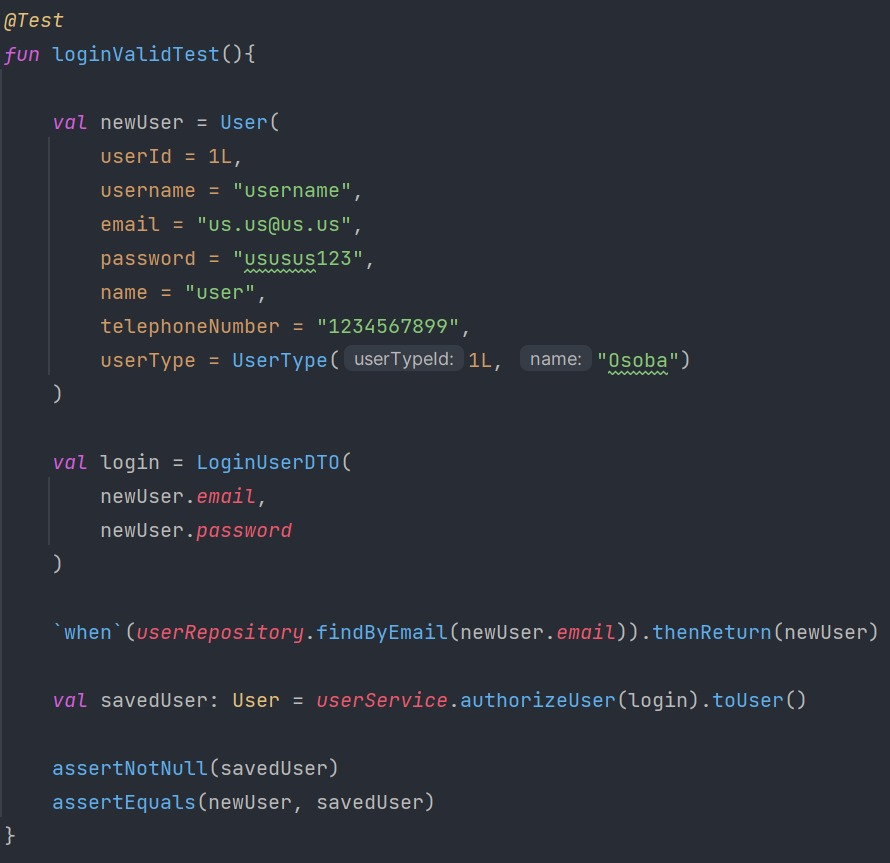
\includegraphics[scale=0.5]{slike/unit1.PNG} 
			\centering
			\caption{Unit test 1 - \textit{log-in}}
			\label{unit1}
		\end{figure}

\pagebreak
\textbf{Ispitni slučaj 2: Drugi test provjerava prijavu s neispravnom lozinkom.}

		\begin{figure}[H]
			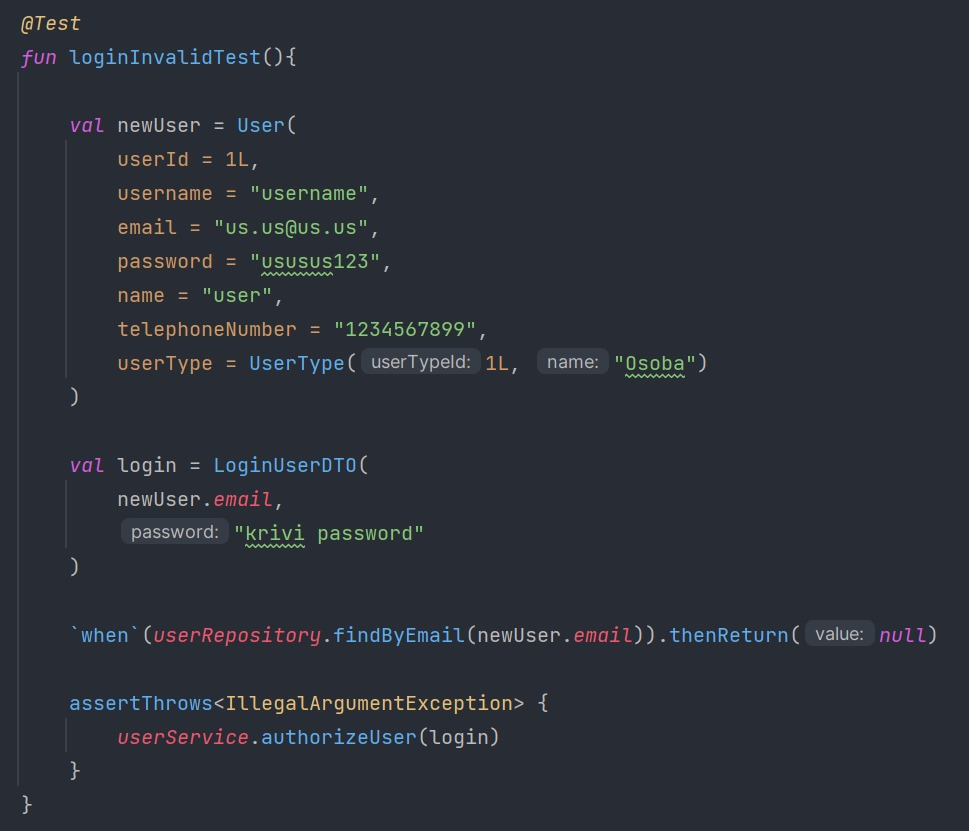
\includegraphics[scale=0.5]{slike/unit2.PNG} 
			\centering
			\caption{Unit test 2 - \textit{log-in} s neispravnom lozinkom.}
			\label{unit2}
		\end{figure}

\pagebreak		
\textbf{Ispitni slučaj 3: Treći test provjerava uspješnu registraciju.}

		\begin{figure}[H]
			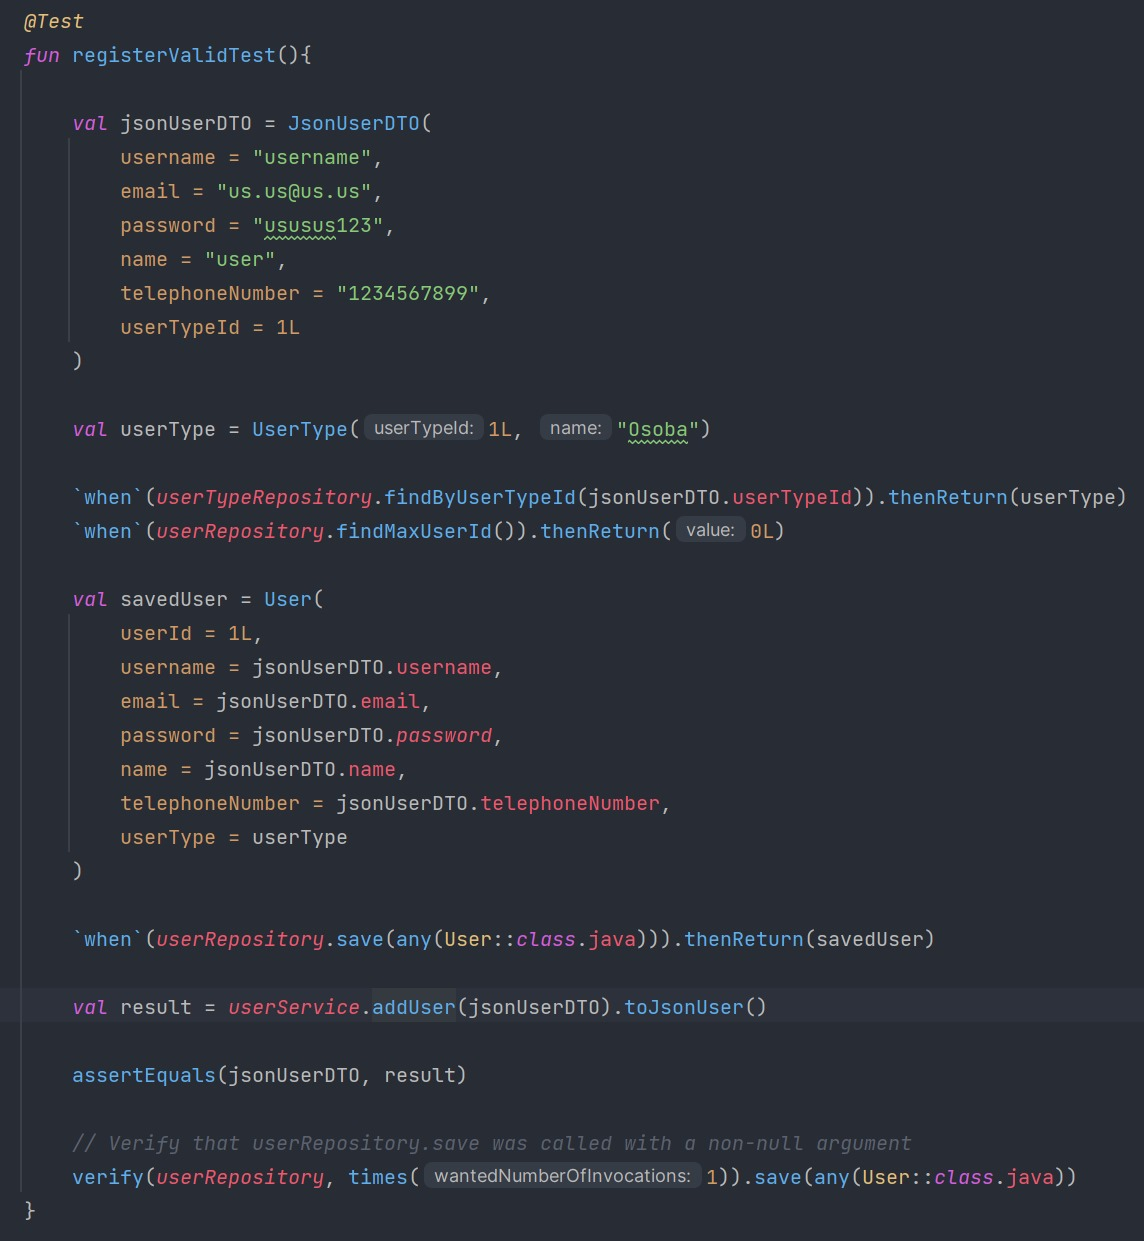
\includegraphics[scale=0.5]{slike/unit3.PNG} 
			\centering
			\caption{Unit test 3 - registracija}
			\label{unit3}
		\end{figure}
		
\pagebreak		
\textbf{Ispitni slučaj 4: U četvrtom testu testiramo pokušaj registracije s \textit{e-mail}-om koji je već u uporabi.}

		\begin{figure}[H]
			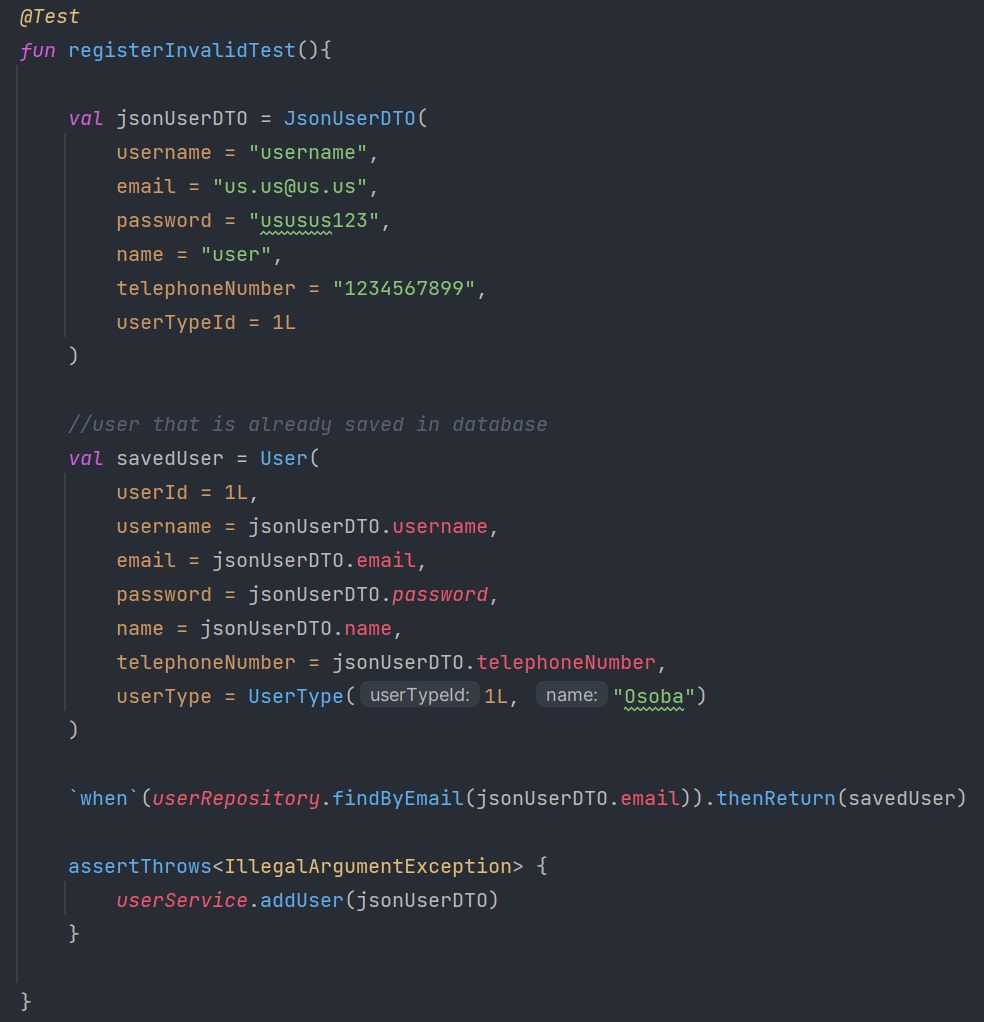
\includegraphics[scale=0.5]{slike/unit4.PNG} 
			\centering
			\caption{Unit test 4 - registracija s već postojećim \textit{e-mail}-om}
			\label{unit4}
		\end{figure}

\pagebreak		
\textbf{Ispitni slučaj 5: Peti test testira rutu dohvaćanja svih korisnika koji su prijavljeni kao sklonište odnosno "shelter".}

		\begin{figure}[H]
			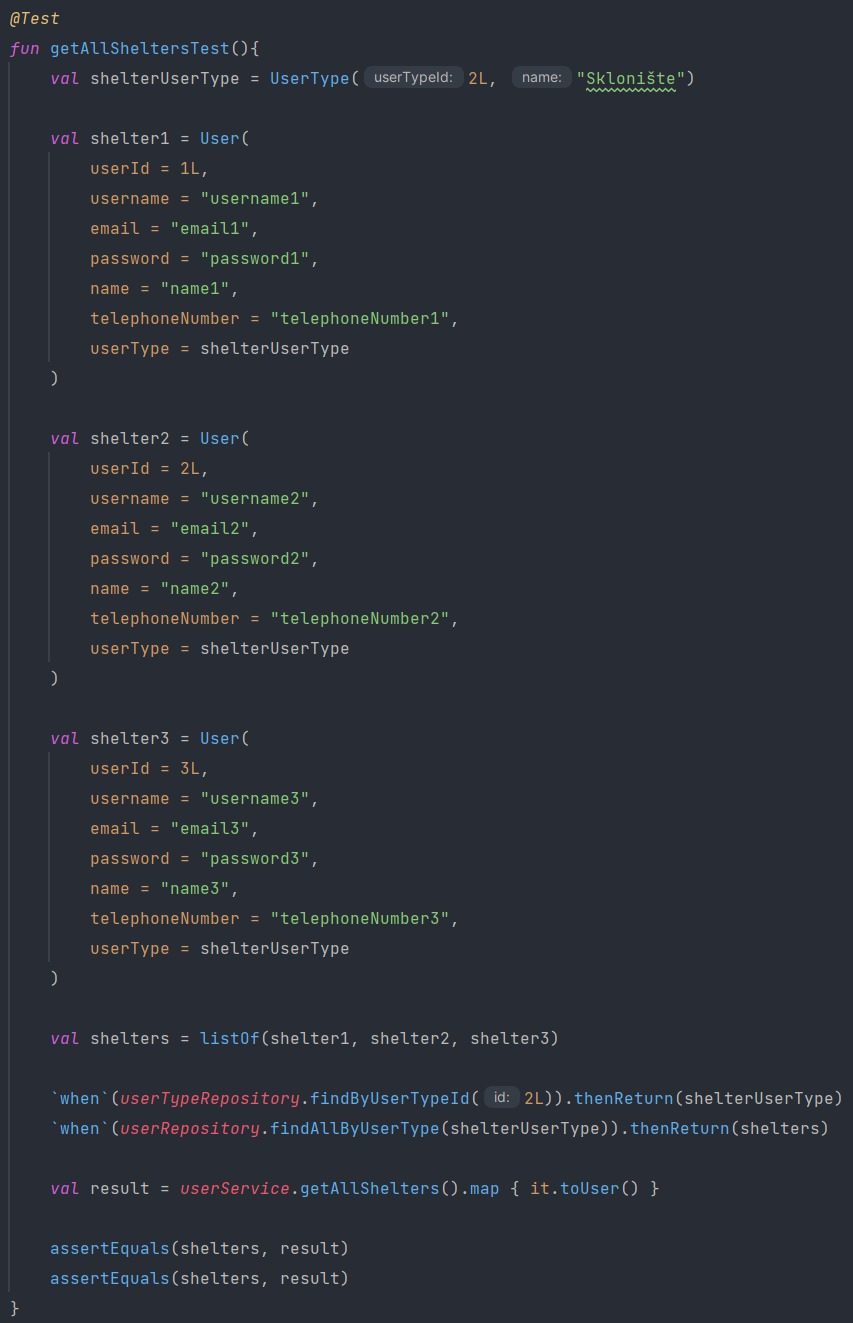
\includegraphics[scale=0.5]{slike/unit5.PNG} 
			\centering
			\caption{Unit test 5 - ruta dohvaćanja svih korisnika}
			\label{unit5}
		\end{figure}
		
\pagebreak
\textbf{Ispitni slučaj 6: U šestom testu testiramo dodavanje novog oglasa.}		
		
		\begin{figure}[H]
			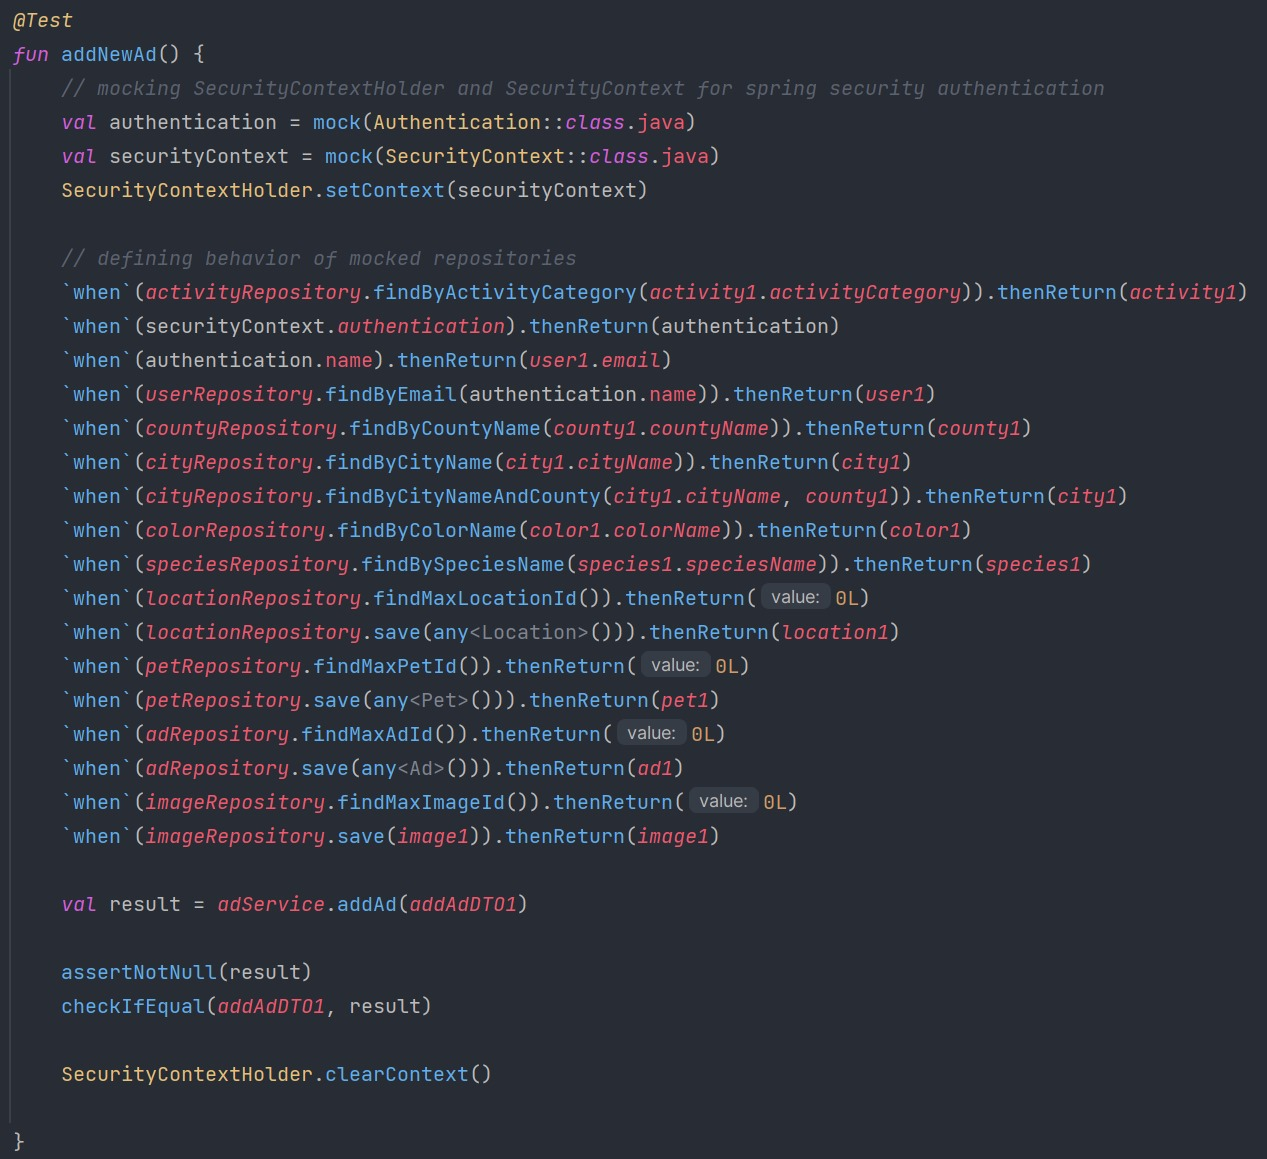
\includegraphics[scale=0.5]{slike/unit6.PNG} 
			\centering
			\caption{Unit test 6 - dodavanje novog oglasa}
			\label{unit6}
		\end{figure}

\pagebreak
		
\textbf{Prikaz rezultata unit testova}\\

Prvih 5 unit testova (loginValidTest, loginInvalidTest, registerValidTest, registerInvalidTest i getAllSheltersTest) služi za testiranje metoda iz UserService-a. Svi testovi su bili uspješni.

		\begin{figure}[H]
			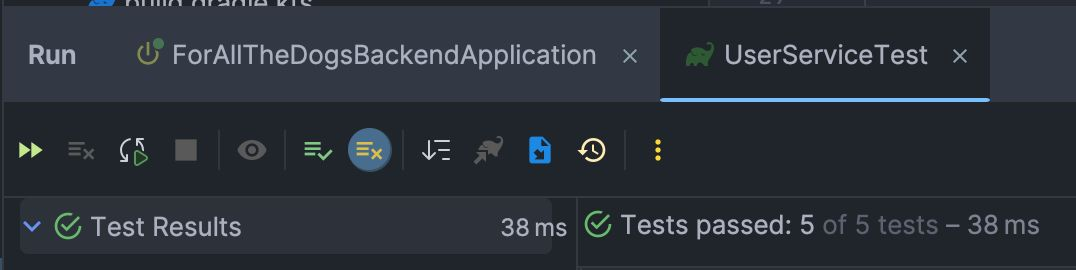
\includegraphics[scale=0.45]{slike/5unitrez.PNG} 
			\centering
			\caption{Prikaz prolaznosti unit testova (1. - 5.)}
			\label{5unitrez}
		\end{figure}
		
		
Zadnji test (addNewAd) služi za testiranje metode iz AdService-a koja omogućuje dodavanje novog oglasa. Test je također bio uspješan.

		\begin{figure}[H]
			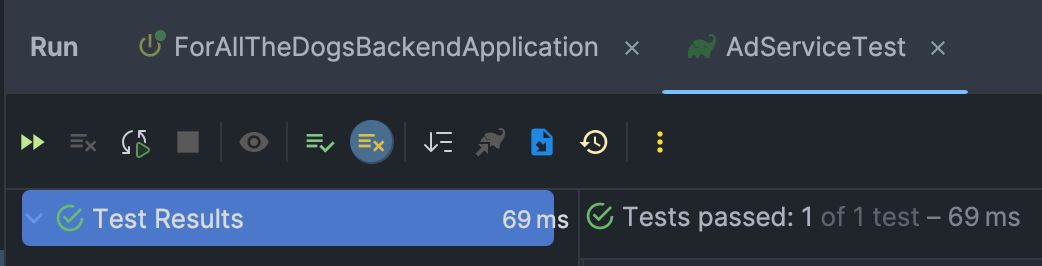
\includegraphics[scale=0.45]{slike/1unitrez.PNG} 
			\centering
			\caption{Prikaz prolaznosti 6. unit testa}
			\label{1unitrez}
		\end{figure}
		
\eject
	
			\subsection{Ispitivanje sustava}
			
			Ispitivanje sustava je vrsta softverskog testiranja koja se fokusira na ispitivanje i provjeru cjelokupnog sustava kako bi se omogućilo da svi njegovi dijelovi funkcioniraju zajedno prema specifikacijama i očekivanjima. Kako bismo to postigli u projektu smo koristili radni okvir \textit{WebDriverIO} koji je baziran na Selenium WebDriver-u  te pruža jednostavan i efikasan način za automatizaciju testova web stranica i aplikacija.\\
			
			\textbf{Ispitni slučaj 1: provjera ispravnosti registracije}
			
			Ovaj system test provjerava ispravnost sustava registracije. Korisnik odlazi na glavnu stranicu i čeka dok se ne pojavi gumb za sign-up. Tada ga klikne, ispuni podatke za registraciju (username, e-mail, password, ime i broj telefona) i označi tip korisnika, a zatim klikne gumb za predaju (submit). Na samom kraju se provjerava ispravnost dobivenog URL-a koji nam govori o uspješnosti registracije.\\
			
			\textbf{Ulaz:}

				\begin{enumerate}
					\item Unos svih ispravnih podataka
					\item Izostavljen unos username-a
					\item Izostavljen unos e-mail-a
				\end{enumerate}
				
			\textbf{Očekivani rezultat:}
			
				\begin{enumerate}
					\item Nije došlo do greške - svi su podaci uspješno uneseni.
					\item Došlo je do greške. I dalje smo na sign-up dijelu dok se ne unesu svi podaci ispravno.
					\item Došlo je do greške. I dalje smo na sign-up dijelu dok se ne unesu svi podaci ispravno.
				\end{enumerate}
			
			\begin{figure}[H]
				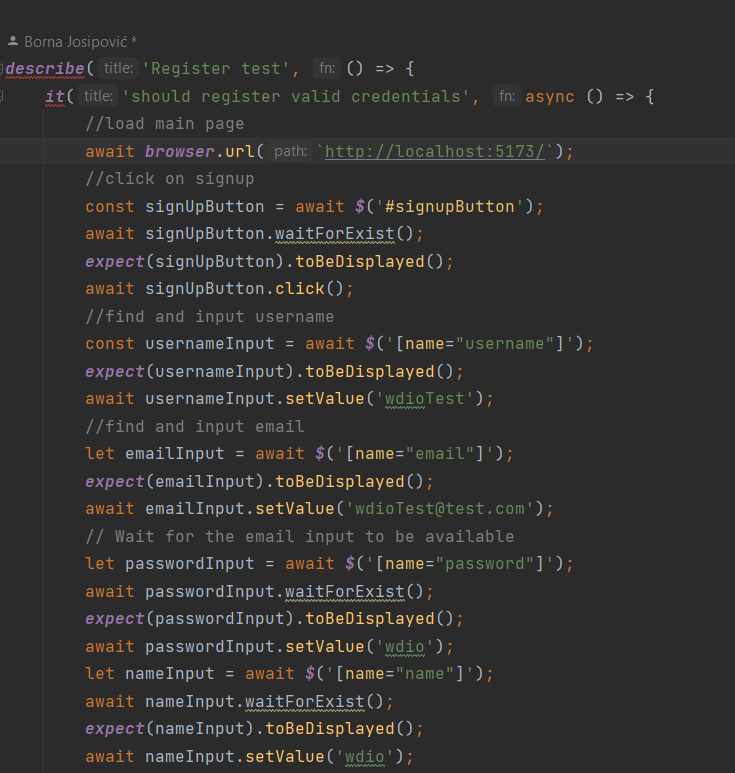
\includegraphics[scale=0.7]{slike/sysreg1.PNG} 
				\centering
				\caption{System test: ispravan unos podataka pri registraciji (1.)}
				\label{sysreg1}
			\end{figure}
			
			\begin{figure}[H]
				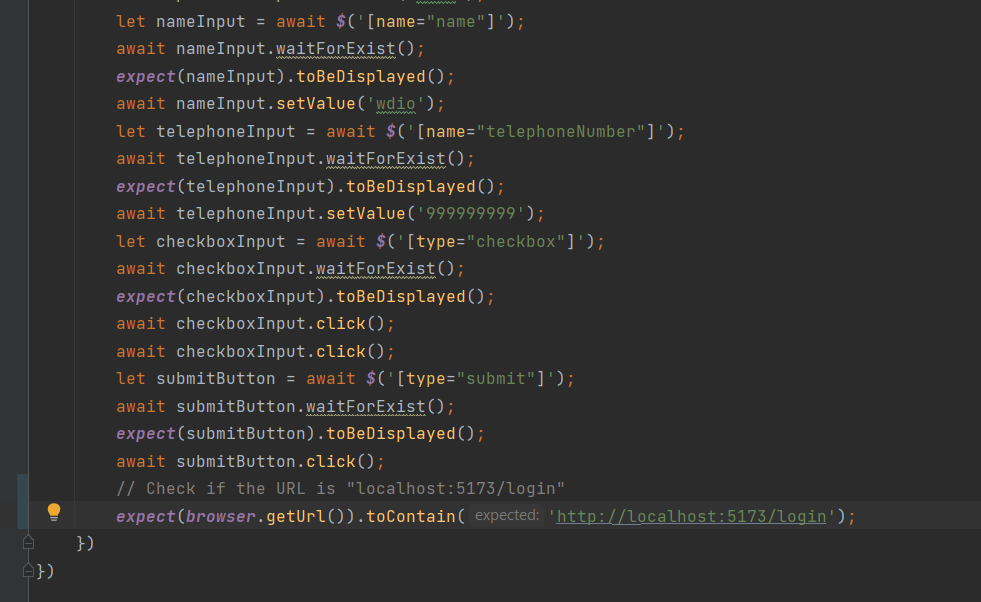
\includegraphics[scale=0.7]{slike/sysreg2.PNG} 
				\centering
				\caption{System test: ispravan unos podataka pri registraciji (2.)}
				\label{sysreg2}
			\end{figure}
			
			\textbf{Rezultat:}
			Svi su rezultati testova jednaki očekivanim.\\
			
			\textbf{Ispitni slučaj 2: provjera ispravnosti ulogiravanja}
			
			Ovaj system test provjerava ispravnost sustava ulogiravanja. Korisnik čeka dok se ne pojavi gumb za log-in, a kad se pojavi unosi svoj e-mail i password. Zatim klikne gumb za predaju te se odvija provjera ispravnosti dobivenog URL-a. Nakon toga se prepoznaje i dohvaća username korisnika i ispisuje se poruka "Hello, \textit{username}". \\
			
			\textbf{Ulaz:}
			
				\begin{enumerate}
					\item Unos svih ispravnih podataka
					\item Unos e-mail-a koji ne postoji u bazi podataka
					\item Izostavljen unos e-mail-a
				\end{enumerate}
				
			\textbf{Očekivani rezultat:}
			
				\begin{enumerate}
					\item Nije došlo do greške - svi su podaci uspješno uneseni.
					\item Došlo je do greške i ispisa "Wrong Credentials!" pri predaji promjena (submit).
					\item Došlo je do greške. I dalje smo na log-in dijelu dok se ne unesu svi podaci ispravno.
				\end{enumerate}
			
			\begin{figure}[H]
				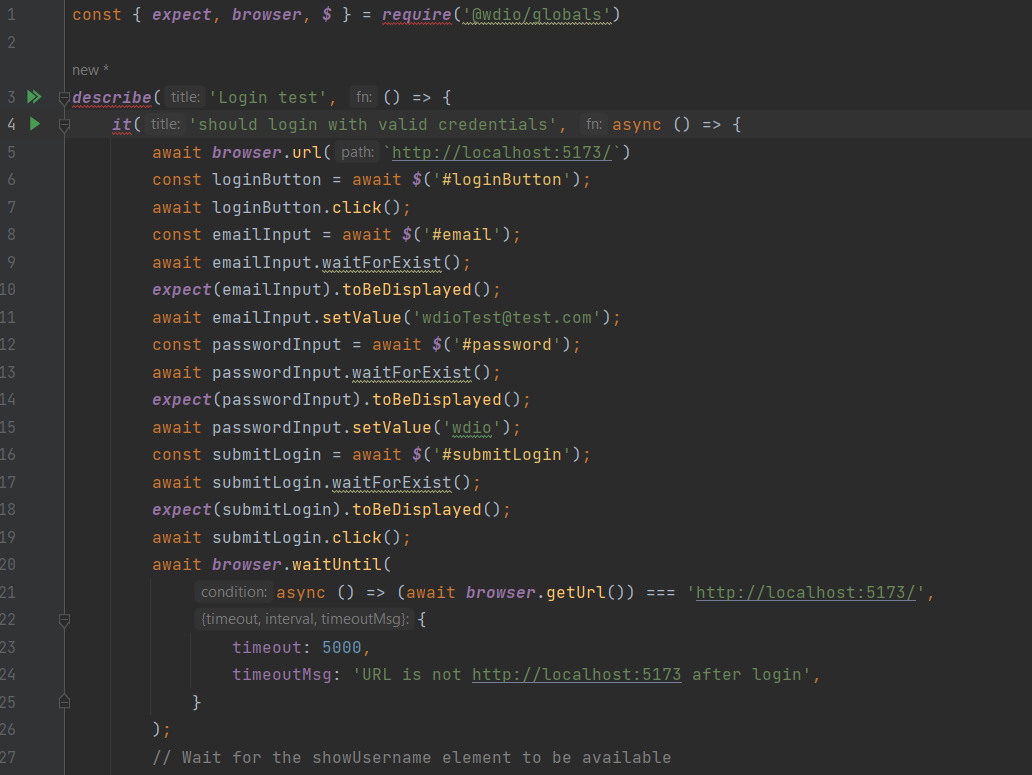
\includegraphics[scale=0.7]{slike/syslogin1.PNG} 
				\centering
				\caption{System test: ispravan unos podataka pri ulogiravanju (1.)}
				\label{syslogin1}
			\end{figure}
			
			\begin{figure}[H]
				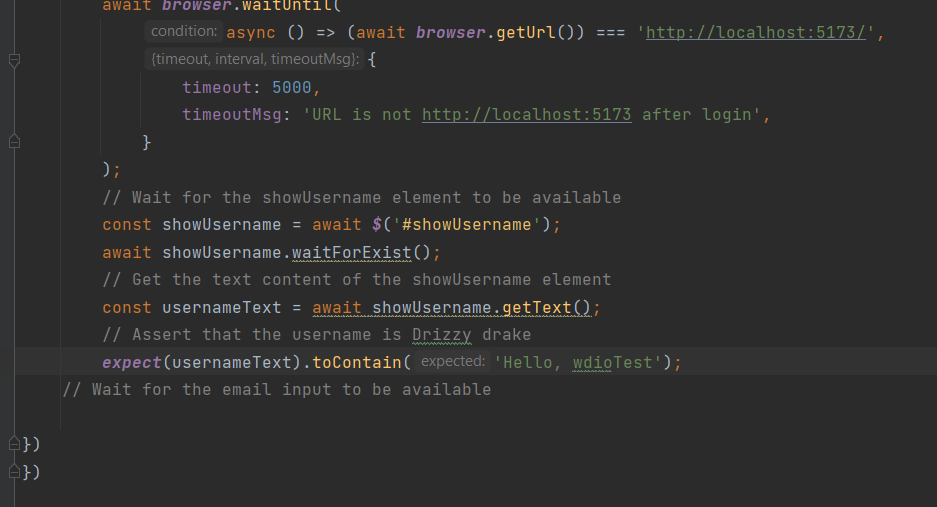
\includegraphics[scale=0.7]{slike/syslogin2.PNG} 
				\centering
				\caption{System test: ispravan unos podataka pri ulogiravanju (2.)}
				\label{syslogin2}
			\end{figure}
			
			\textbf{Rezultat:}
			Svi su rezultati testova jednaki očekivanim.\\
			
			\textbf{Ispitni slučaj 3: provjera ispravnosti izmjene oglasa}
			
			Ovaj system test provjerava ispravnost sustava izmjene oglasa. Pronalazi se post korisnika, a zatim se ulazi u ekran za izmjenu oglasa. Korisnik izvodi promjene u oglasu i klikne gumb za predaju. Uspoređuje se tekst iz oglasa na glavnoj stranici o izmijenjenom podatku s novom vrijednosti podatka. Ako su identični, izmjena je uspjela. \\
			
			\textbf{Ulaz:}
			
				\begin{enumerate}
					\item Promijenjena je vrsta životinje iz "Pas" u "Papiga" i pohranjuje se ta promjena
					\item Brisanje jedine slike unutar oglasa
				\end{enumerate}
				
			\textbf{Očekivani rezultat:}
			
				\begin{enumerate}
					\item Nije došlo do greške - promjena je uspjela.
					\item Došlo je do greške i ispisa "At least 1 image!" pri predaji promjena (submit).
				\end{enumerate}
			
			\begin{figure}[H]
				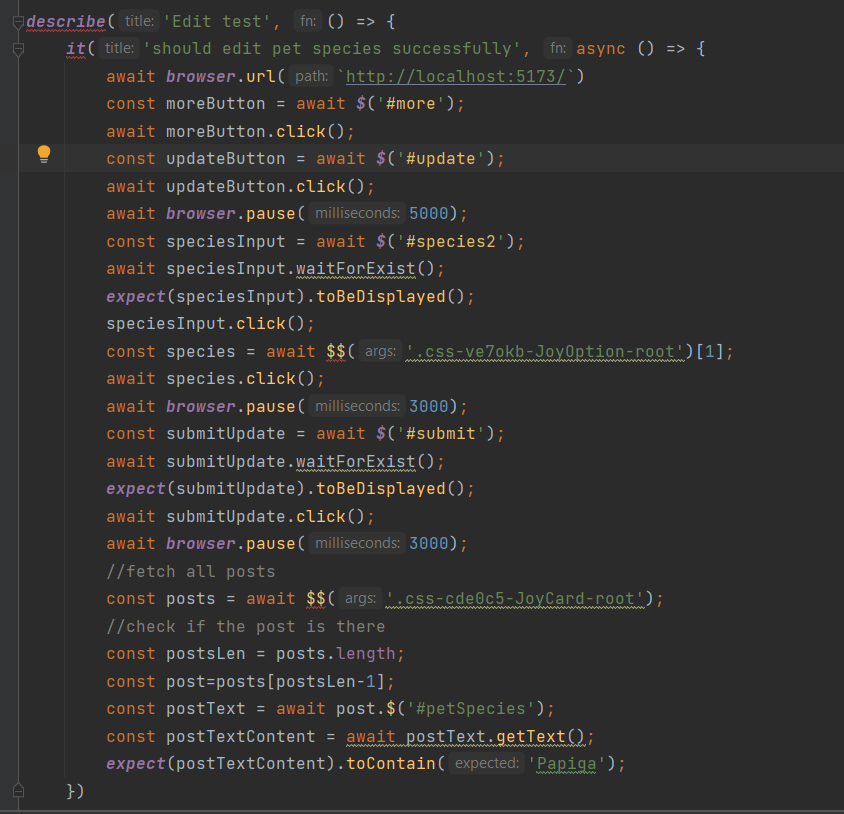
\includegraphics[scale=0.7]{slike/sysedit1.PNG} 
				\centering
				\caption{System test: promjena vrste životinje iz "Pas" u "Papiga" na oglasu}
				\label{sysedit1}
			\end{figure}
			
			
			\begin{figure}[H]
				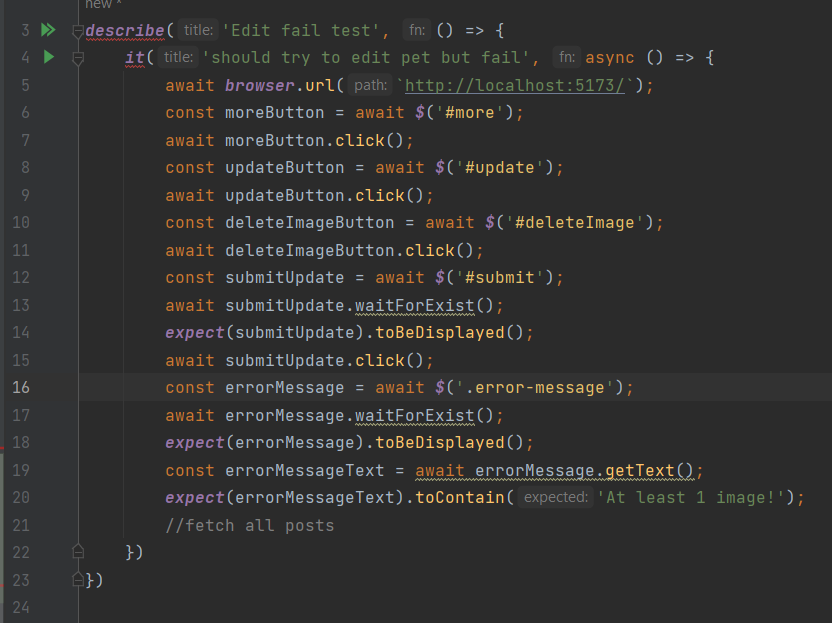
\includegraphics[scale=0.7]{slike/sysedit2.PNG} 
				\centering
				\caption{System test: pokušaj brisanja jedine slike unutar oglasa}
				\label{sysedit2}
			\end{figure}
			
			\textbf{Rezultat:}
			Svi su rezultati testova jednaki očekivanim.\\
			
			\textbf{Ispitni slučaj 4: provjera ispravnosti brisanja postojećeg oglasa}
			
			Ovaj system test provjerava ispravnost sustava brisanja oglasa. Korisnik pronalazi svoj oglas koji namjerava obrisati. Klikne na gumb "3 točke" te se otvaraju opcije manevriranja oglasom i izabire opciju "Delete". Pregledavaju se sva imena objava i ako ne postoji ime upravo obrisane objave među njima onda objava i je obrisana. \\
			
			\textbf{Ulaz:}
			
				\begin{enumerate}
					\item Prikaz testiranja brisanja postojećeg oglasa
				\end{enumerate}
				
			\textbf{Očekivani rezultat:}
			
				\begin{enumerate}
					\item Nije došlo do greške - oglas je uspješno obrisan.
				\end{enumerate}
			
			\begin{figure}[H]
				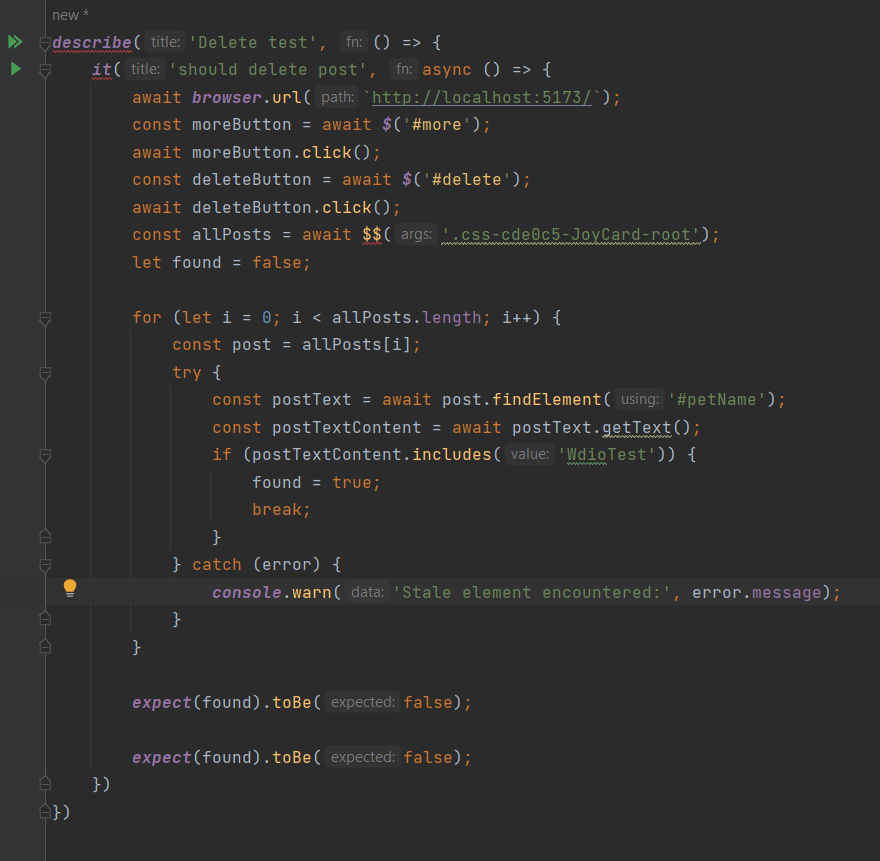
\includegraphics[scale=0.7]{slike/sysdeletepost.PNG} 
				\centering
				\caption{System test: prikaz brisanja postojećeg oglasa}
				\label{sysdeletepost}
			\end{figure}
			
			
			\textbf{Rezultat:}
			Rezultat testa je jednak očekivanom.\\
			
			\textbf{Ispitni slučaj 5: provjera ispravnosti odjave korisničkog računa}
			
			Ovaj system test provjerava ispravnost sustava odjave korisničkog računa. Korisnik klikne na gumb za odjavu (sign-out). Zatim se provjerava postojanje teksta koji se ispisuje na ekranu kada korisnik nije prijavljen ("Please login or signup") što potvrđuje da u tom trenutku nema prijavljenog korisnika. \\
			
			\textbf{Ulaz:}
			
				\begin{enumerate}
					\item Prikaz testiranja odjave korisničkog računa
				\end{enumerate}
				
			\textbf{Očekivani rezultat:}
			
				\begin{enumerate}
					\item Nije došlo do greške - korisnik se uspješno odjavio.
				\end{enumerate}
			
			\begin{figure}[H]
				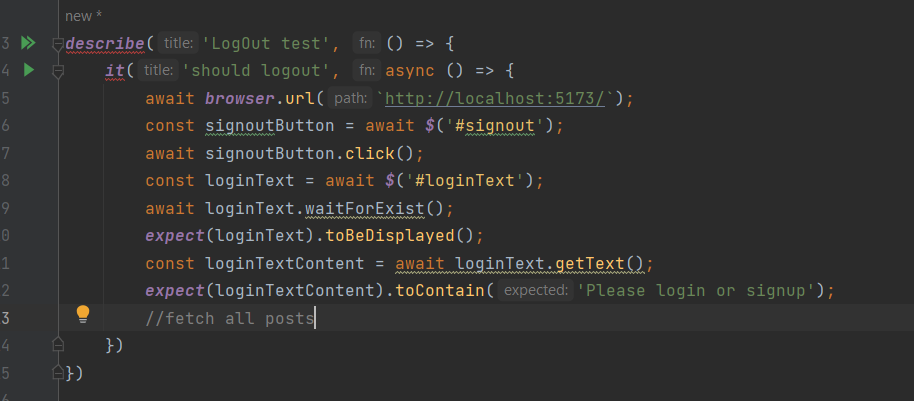
\includegraphics[scale=0.7]{slike/syslogout.PNG} 
				\centering
				\caption{System test: prikaz odjave postojećeg računa}
				\label{syslogout}
			\end{figure}
			
			
			\textbf{Rezultat:}
			Rezultat testa je jednak očekivanom.\\
			
			\eject 
		
		
		\section{Dijagram razmještaja}
			
			Sustav se zasniva na arhitekturi "klijent - poslužitelj". Klijenti koriste web preglednik za pristupanje web aplikaciji. Komunikacija klijenata i poslužitelja odvija se preko HTTP veze. Za posluživanje se koristi platforma Render.
			 
			 \begin{figure}[H]
				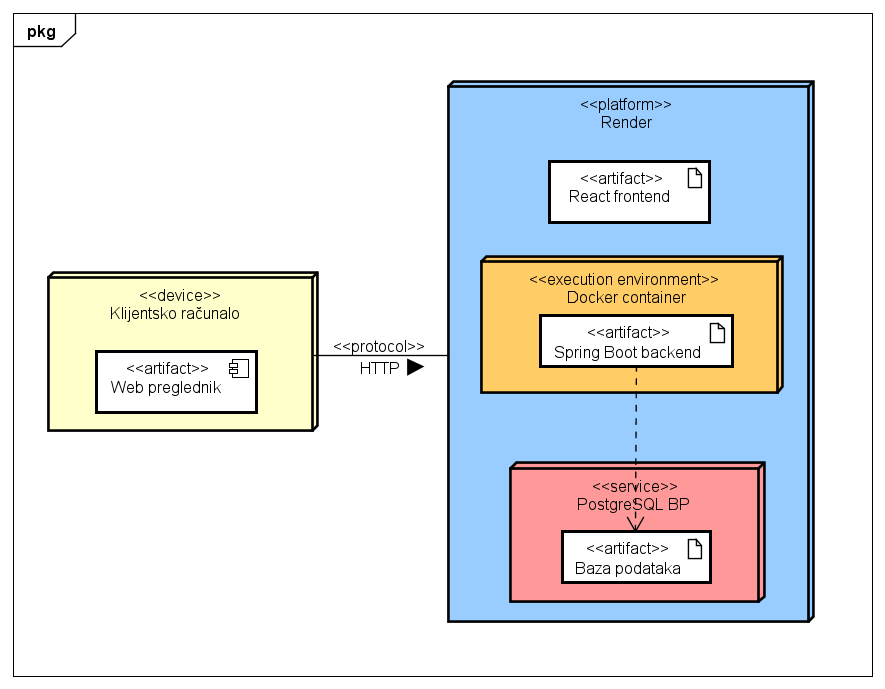
\includegraphics[scale=0.6]{slike/dijagram_razmjestaja.PNG} 
				\centering
				\caption{Dijagram razmještaja}
				\label{dijagram_razmjestaja}
			\end{figure}
			
			\eject 
		
		\section{Upute za puštanje u pogon}
		
			Izvorni kod aplikacije postavljen je na GitHub repozitorij na adresi \url{https://github.com/Ljubimci-Grupa-1/ForAllTheDogs}. Puštanje u pogon obavit ćemo uz pomoć platforme Render\footnote{\url{https://render.com}}.
			
			\subsection{Frontend}
			
			U datoteku \textbf{package.json} dodajemo "dotenv", "express" i "http-proxy-middleware" ovisnosti (engl. \textit{dependencies}) kao što je prikazano na slici \ref{dependencies}.
			
			\begin{figure}[H]
				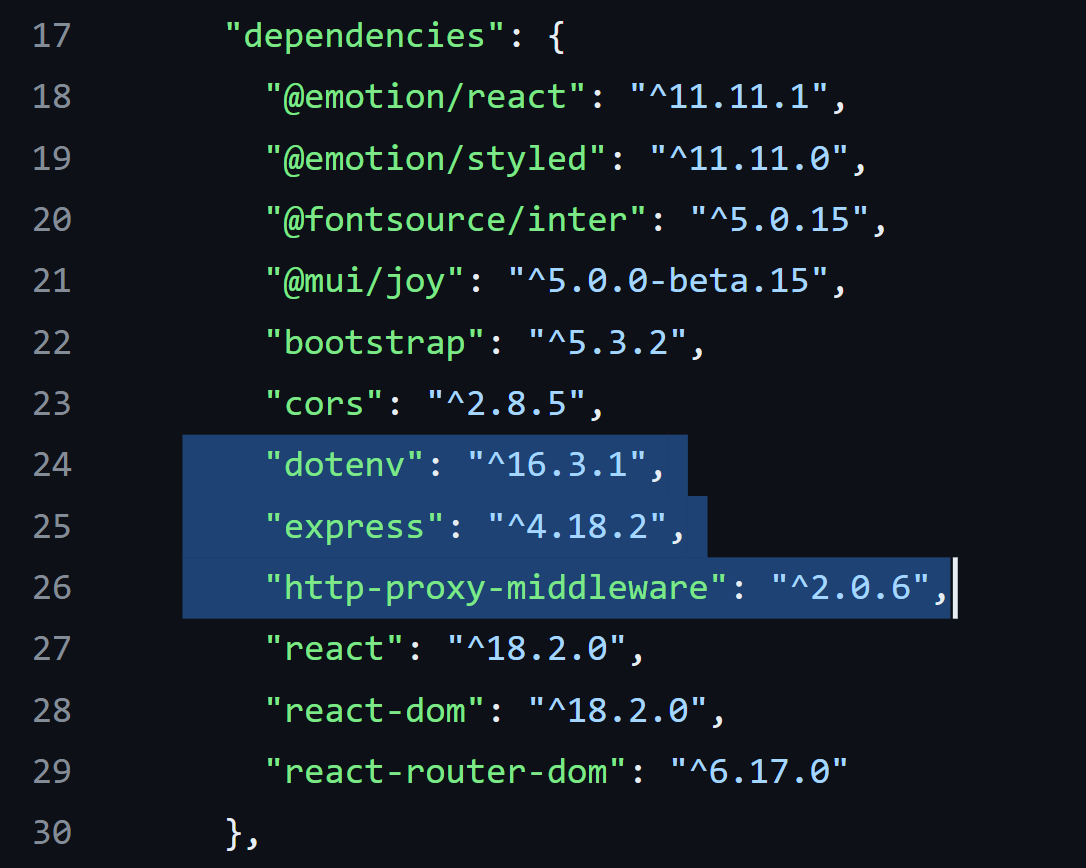
\includegraphics[scale=0.6]{slike/dependencies.PNG} 
				\centering
				\caption{"dependencies" u package.json}
				\label{dependencies}
			\end{figure}
			
			Datoteku \textbf{server.js}, prikazanu na slici \ref{server_js}, stavljamo u korijenski direktorij za frontend. Ona sadrži konfiguraciju za Express server koji koristimo za posluživanje frontenda.
			
			\begin{figure}[H]
				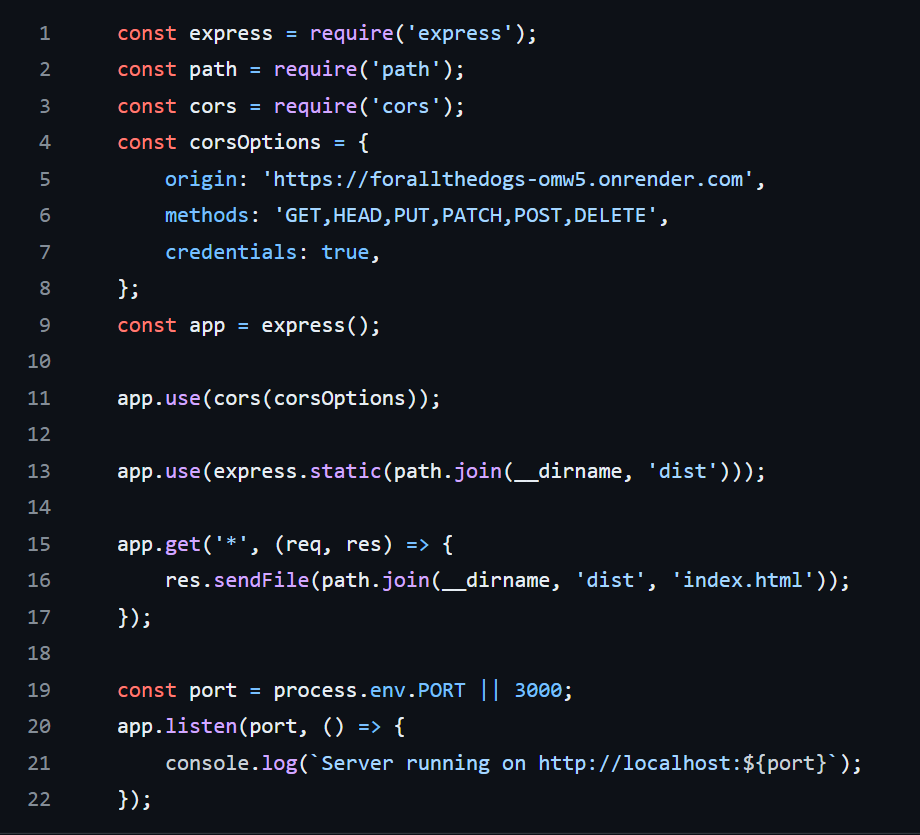
\includegraphics[scale=0.6]{slike/server_js.PNG} 
				\centering
				\caption{Sadržaj datoteke server.js}
				\label{server_js}
			\end{figure}
			
			Zatim se vraćamo u datoteku \textbf{package.json} i ažuriramo "scripts" kao na slici \ref{scripts} te obavimo \textit{git push}.
			
			\begin{figure}[H]
				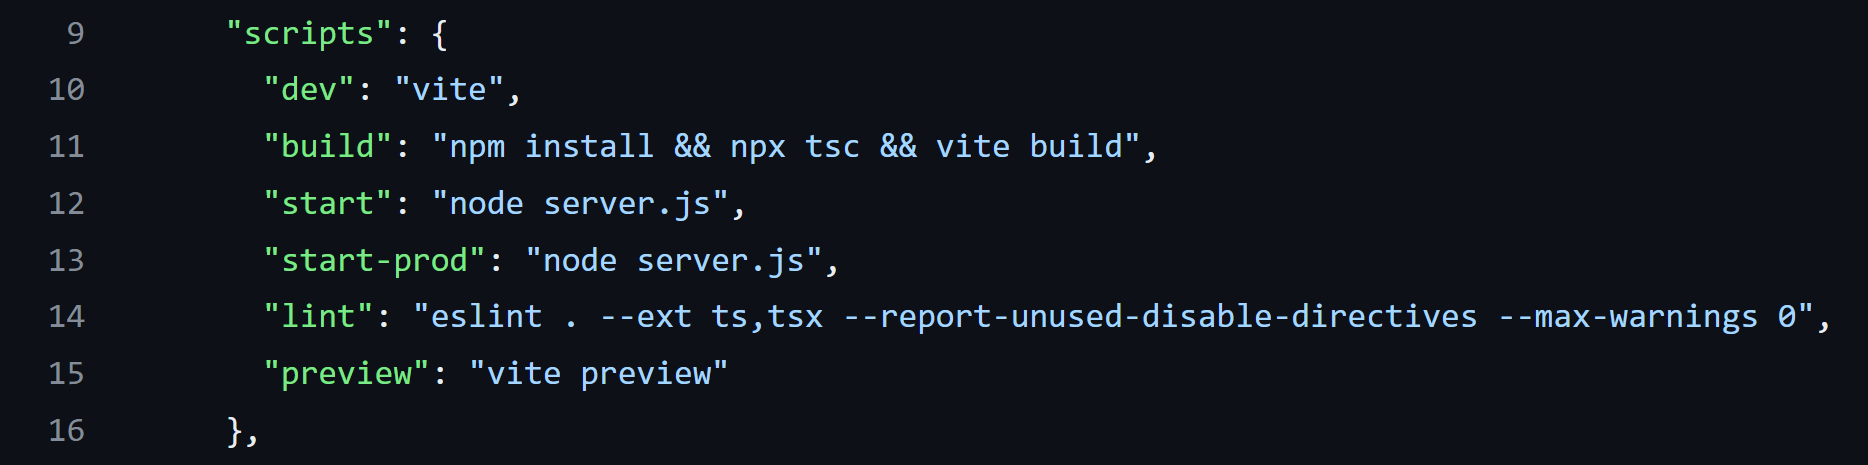
\includegraphics[scale=0.4]{slike/scripts.PNG} 
				\centering
				\caption{"scripts" u package.json}
				\label{scripts}
			\end{figure}
			
			Prijavljujemo se na \url{https://dashboard.render.com} svojim korisničkim podacima te odabiremo \textit{New} $\rightarrow$ \textit{Web Service}. Nakon odabira našeg GitHub repozitorija postavljamo željeno ime, regiju (EU Central), odgovarajuću granu repozitorija (main), te ime korijenskog direktorija za frontend dio aplikacije (direktorij \textbf{frontend}).
			
			\begin{figure}[H]
				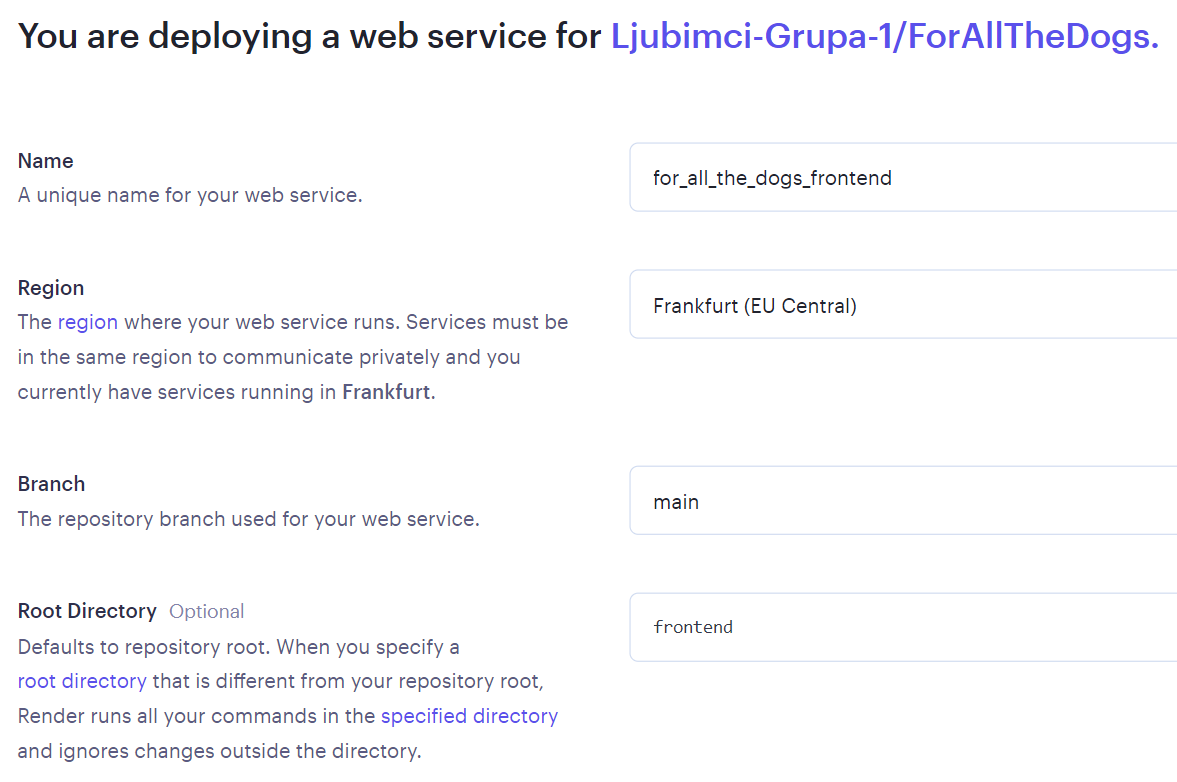
\includegraphics[scale=0.6]{slike/frontend_1.PNG} 
				\centering
				\caption{Postavljanje Web Service}
				\label{frontend_1}
			\end{figure}
			
			Nadalje navodimo \textit{Build} i \textit{Start} naredbe koje će biti pokrenute u odabranom korijenskom direktoriju. Naredba \textit{Build} (u našem slučaju \textit{yarn build}) odgovorna je za instalaciju potrebnih programskih biblioteka i kompilaciju koda (uz automatski \textit{redeployment} prilikom svake promjene izvornog koda na GitHub repozitoriju). Naredba \textit{Start} (u našem slučaju \textit{yarn start-prod}) služi za pokretanje aplikacije odnosno web poslužitelja.
			
			\begin{figure}[H]
				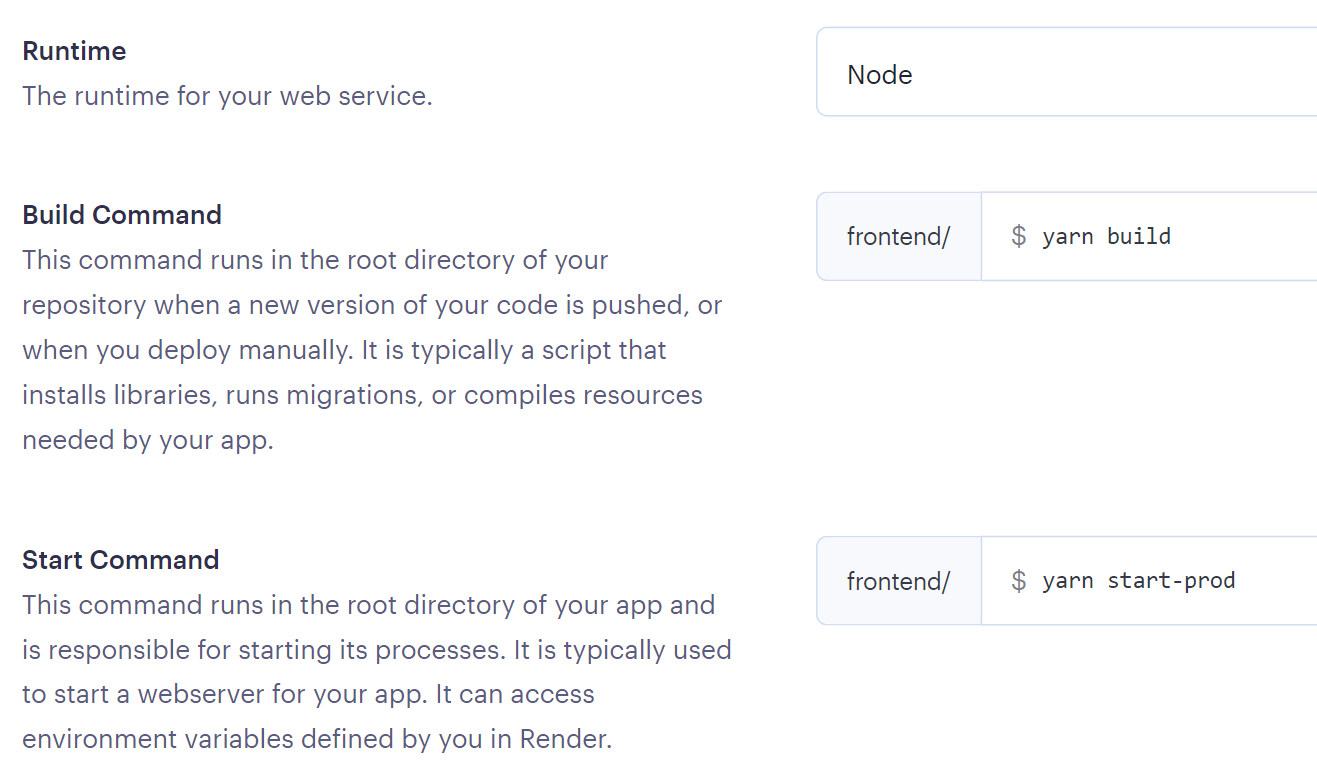
\includegraphics[scale=0.6]{slike/frontend_2.PNG} 
				\centering
				\caption{Build i Start}
				\label{frontend_2}
			\end{figure}
			
			Za kraj odabiremo opciju \textit{Create Web Service}.
			
			\subsection{Baza podataka}
			
			Na Render Dashboard odabiremo \textit{New} $\rightarrow$ \textit{PostgreSQL}. Ispunjavamo željene postavke (ime, regija, PostgreSQL verzija (15) itd.) te završavamo s \textit{Create Database}.
			
			\subsection{Backend}
			
			Za puštanje backenda u pogon ponovno odabiremo \textit{New} $\rightarrow$ \textit{Web Service} te kao korijenski direktorij odabiremo direktorij \textbf{backend}.
			
			\begin{figure}[H]
				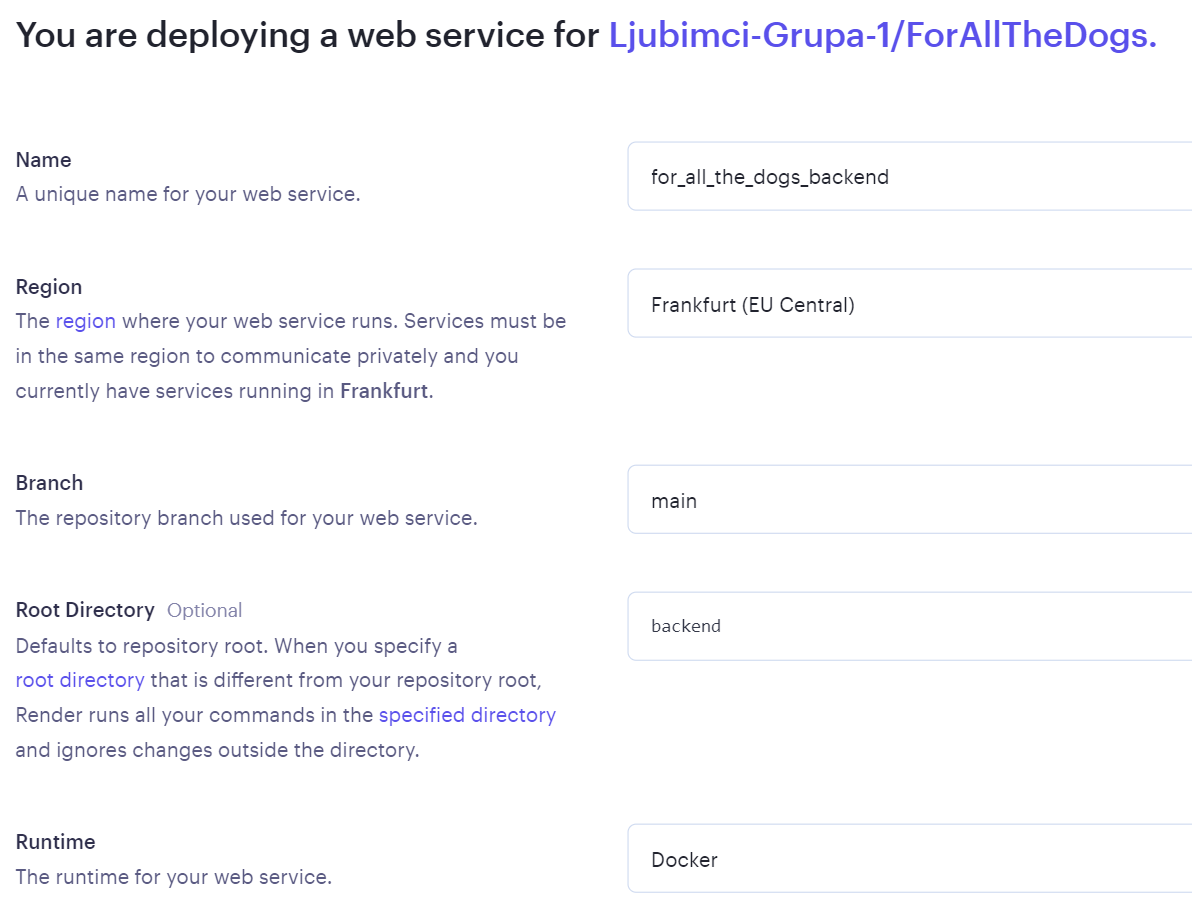
\includegraphics[scale=0.6]{slike/backend.PNG} 
				\centering
				\caption{Postavke za backend}
				\label{backend}
			\end{figure}
			
			Kao \textit{Runtime} postavljamo Docker. Datoteka Dockerfile, pozicionirana u korijenskom direktoriju za backend, sadrži instrukcije za izgradnju i pakiranje (engl. \textit{build-and-package}) aplikacije. Objasnimo sadržaj datoteke Dockerfile.
			
			Prvo se definira "builder".
			
			\begin{figure}[H]
				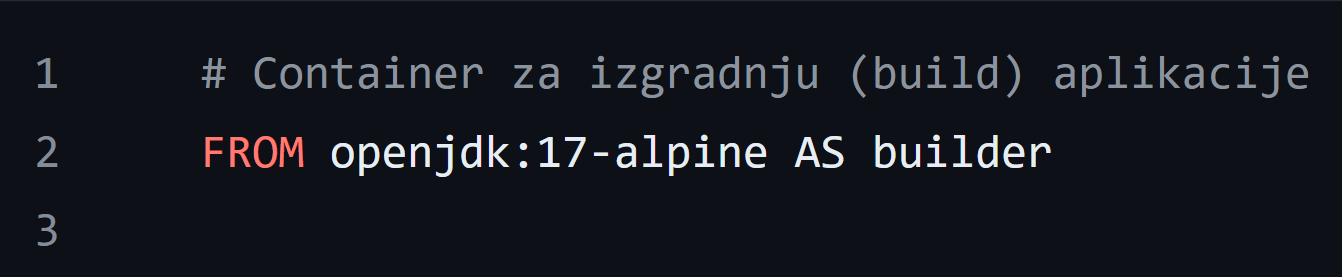
\includegraphics[scale=0.5]{slike/dockerfile_builder.PNG} 
				\centering
				\caption{builder}
				\label{dockerfile_builder}
			\end{figure}
			
			Zatim se zadaje radni direktorij te u kontejner kopira konfiguracijske datoteke alata Gradle (\textbf{build.gradle.kts} i \textbf{settings.gradle.kts}), skripte Gradle omotača (\textit{Gradle Wrapper}) te izvorni kod aplikacije.
			
			\begin{figure}[H]
				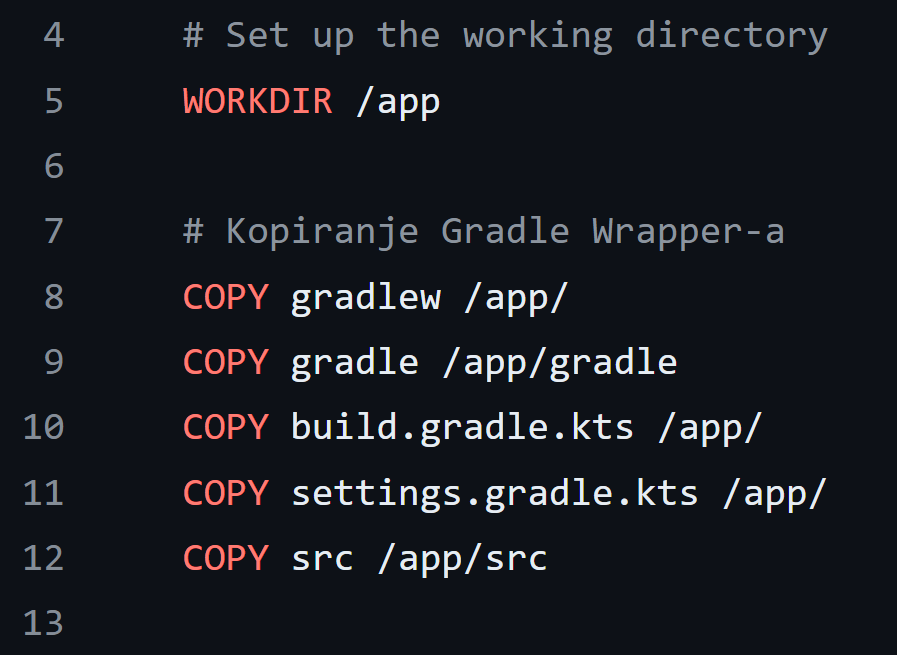
\includegraphics[scale=0.6]{slike/dockerfile_workdir.PNG} 
				\centering
				\caption{Radni direktorij i Gradle}
				\label{dockerfile_workdir}
			\end{figure}
			
			Naredbe na slici \ref{dockerfile_run} (redom) služe za: 
			\begin{packed_item}
				\item davanje skripti Gradle omotača pravo izvršavanja (\textit{execute} permission)
				\item preuzimanje \textit{project dependencies}
				\item izgradnju aplikacije
			\end{packed_item}
			
			\begin{figure}[H]
				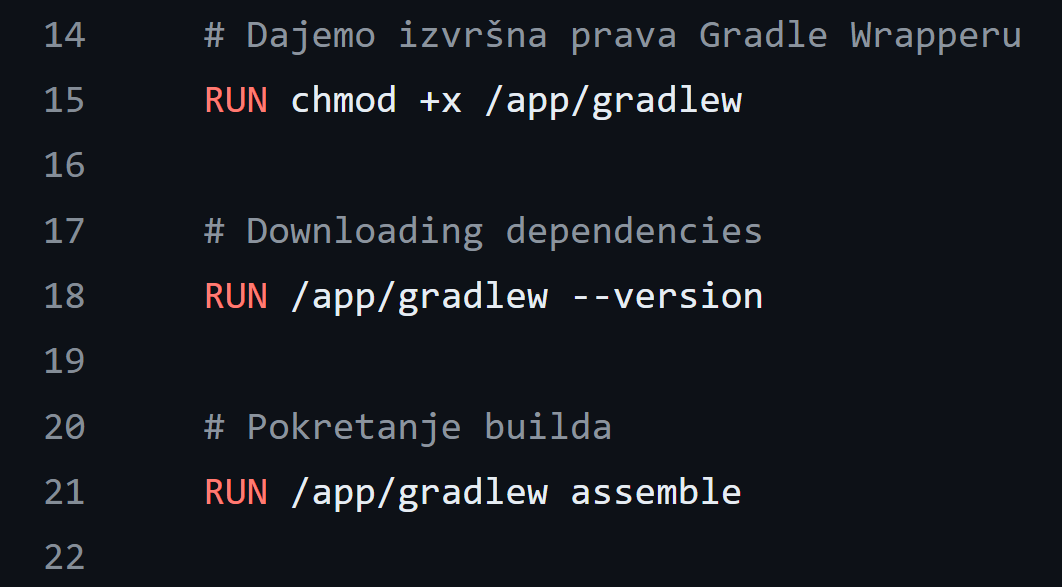
\includegraphics[scale=0.6]{slike/dockerfile_run.PNG} 
				\centering
				\caption{Naredbe za izgradnju}
				\label{dockerfile_run}
			\end{figure}
			
			Na kraju imamo naredbe vezane uz \textit{staging}. Pokrećemo novi \textit{stage} koji koristi istu osnovnu sliku za izvođenje aplikacije (\textit{build stage} više nam nije potreban, kopiraju se samo potrebni artefakti). Izgrađena JAR datoteka (iz \textit{build stage}) kopira se u trenutni \textit{stage}. Zatim su navedene naredbe koje će biti izvedene pri pokretanju kontejnera. Aplikacija se pokreće kao izvršna datoteka (\textit{executable}).
			
			\begin{figure}[H]
				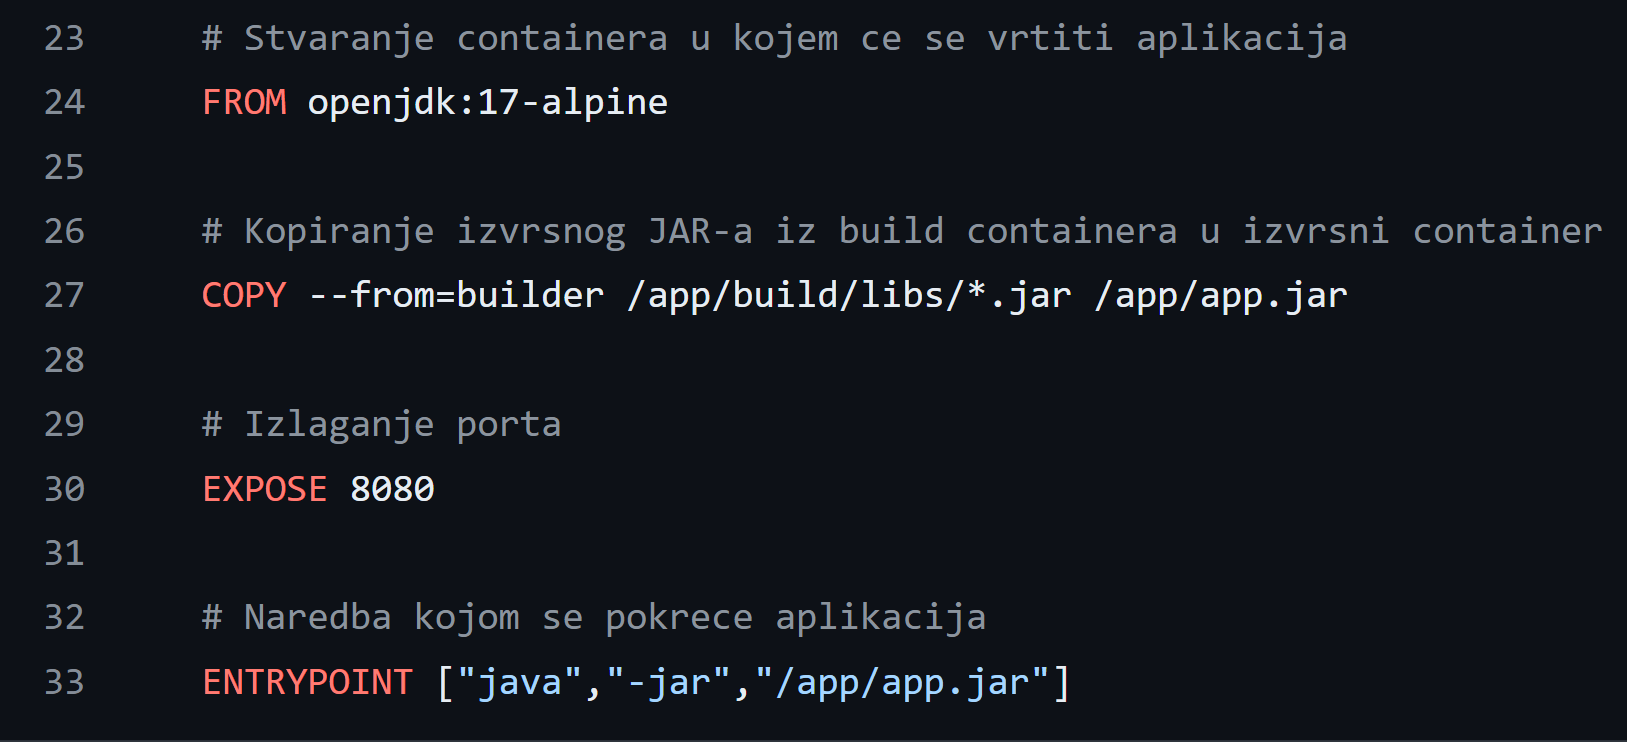
\includegraphics[scale=0.45]{slike/dockerfile_stage.PNG} 
				\centering
				\caption{Naredbe za \textit{staging}}
				\label{dockerfile_stage}
			\end{figure}
			
			Kao i prije, završavamo s \textit{Create Web Service}.
			
			\eject 